\documentclass[tikz]{standalone}

\begin{document}

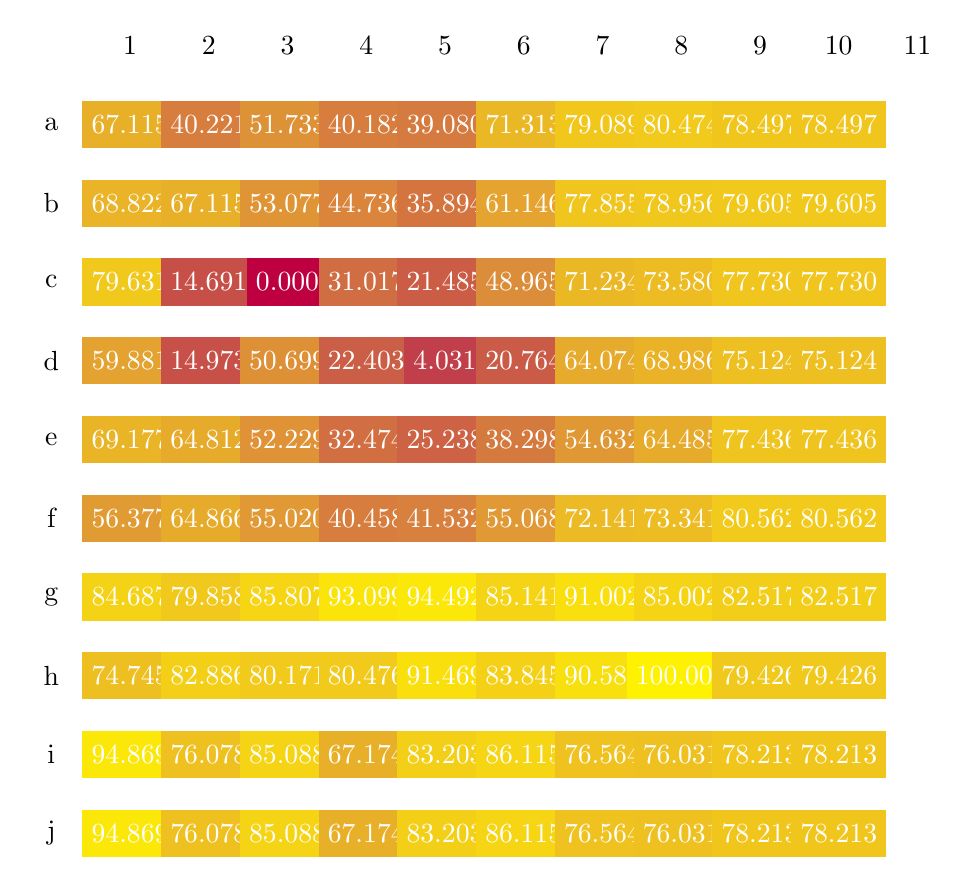
\begin{tikzpicture}
\foreach \y [count=\n] in {
    {67.115,40.221,51.733,40.182,39.080,71.313,79.089,80.474,78.497,78.497},
    {68.822,67.115,53.077,44.736,35.894,61.146,77.855,78.956,79.605,79.605},
    {79.631,14.691,0.000,31.017,21.485,48.965,71.234,73.580,77.730,77.730},
    {59.881,14.973,50.699,22.403,4.031,20.764,64.074,68.986,75.124,75.124},
    {69.177,64.812,52.229,32.474,25.238,38.298,54.632,64.485,77.436,77.436},
    {56.377,64.866,55.020,40.458,41.532,55.068,72.141,73.341,80.562,80.562},
    {84.687,79.858,85.807,93.099,94.492,85.141,91.002,85.002,82.517,82.517},
    {74.745,82.886,80.171,80.476,91.469,83.845,90.589,100.000,79.426,79.426},
    {94.869,76.078,85.088,67.174,83.203,86.115,76.564,76.031,78.213,78.213},
    {94.869,76.078,85.088,67.174,83.203,86.115,76.564,76.031,78.213,78.213},
} {
    \node at (\n, 0) {\n};
    \foreach \x [count=\m] in \y {
        \node[fill=yellow!\x!purple, minimum size=6mm, text=white] at (\m,-\n) {\x};
      }
    }    

% row labels
\foreach \a [count=\i] in {a,b,c,d,e,f,g,h,i,j} {
\node[minimum size=6mm] at (0,-\i) {\a};
}
\end{tikzpicture}
\end{document}